\chapter{Sets, Functions, and Relations}
\pagebreak[4]

\section{Sets and Membership }
\subsection{}
\begin{tcolorbox}
List explicitly the elements of the set 
$$\{x:\,x<0 \text{ and } (x-1)(x+2)(x+3)=0\}$$
\end{tcolorbox}
$$\{\,-3,\, -2\}$$
$$\blacklozenge$$

\subsection{}
\begin{tcolorbox}
List the elements of the set 
$$\{x:\,3x-1  \text{ is a multiple of  } 3\}$$
\end{tcolorbox}
$$\{x:\,x= k+\frac{1}{3},\, k\in \mathbb{Z}\}$$
$$\blacklozenge$$
\subsection{}
\begin{tcolorbox}
Sketch on a number line each of the following sets.\\
(a) $\{x:\,|x-1| \leq 3  \}$\\
(b) $\{x:\,|x-1| \leq 3 \text{ and } |x| \leq 2 \}$\\
(c) $\{x:\,|x-1| \leq 3 \text{ or } |x| \leq 2 \}$
\end{tcolorbox}
\begin{figure}[H]%
    \centering
    \subfloat[]{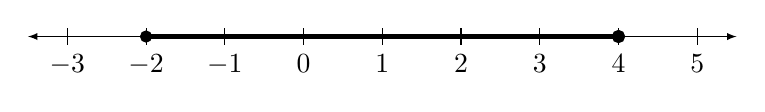
\begin{tikzpicture}
\draw[ultra thick] (-2,0) -- (4,0);
\path [draw=black, fill=black] (-2,0) circle (2pt);
\path [draw=black, fill=black, thick] (4,0.0) circle (2pt);
\draw[latex-latex, very thin] (-3.5,0) -- (5.5,0) ;
\foreach \x in  {-3,-2,-1,0,1,2,3,4,5}
\draw[shift={(\x,0)},color=black] (0pt,3pt) -- (0pt,-3pt);
\foreach \x in {-3,-2,-1,0,1,2,3,4,5}
\draw[shift={(\x,0)},color=black] (0pt,0pt) -- (0pt,-3pt) node[below] 
{$\x$};
\end{tikzpicture}}\\
    \subfloat[]{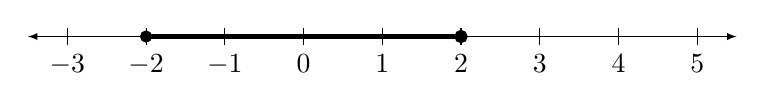
\begin{tikzpicture}
\draw[ultra thick] (-2,0) -- (2,0);
\path [draw=black, fill=black] (-2,0) circle (2pt);
\path [draw=black, fill=black, thick] (2,0.0) circle (2pt);
\draw[latex-latex, very thin] (-3.5,0) -- (5.5,0) ;
\foreach \x in  {-3,-2,-1,0,1,2,3,4,5}
\draw[shift={(\x,0)},color=black] (0pt,3pt) -- (0pt,-3pt);
\foreach \x in {-3,-2,-1,0,1,2,3,4,5}
\draw[shift={(\x,0)},color=black] (0pt,0pt) -- (0pt,-3pt) node[below] 
{$\x$};
\end{tikzpicture}}\\
    \subfloat[]{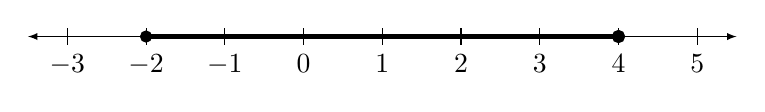
\begin{tikzpicture}
\draw[ultra thick] (-2,0) -- (4,0);
\path [draw=black, fill=black] (-2,0) circle (2pt);
\path [draw=black, fill=black, thick] (4,0.0) circle (2pt);
\draw[latex-latex, very thin] (-3.5,0) -- (5.5,0) ;
\foreach \x in  {-3,-2,-1,0,1,2,3,4,5}
\draw[shift={(\x,0)},color=black] (0pt,3pt) -- (0pt,-3pt);
\foreach \x in {-3,-2,-1,0,1,2,3,4,5}
\draw[shift={(\x,0)},color=black] (0pt,0pt) -- (0pt,-3pt) node[below] 
{$\x$};
\end{tikzpicture}}\\
%\caption{}
\label{fig:fig_p3}
\end{figure}
$$\blacklozenge$$
\newpage
\section{Some remarks on the use of the connectives \textit{and, or, implies}}
\subsection{}
\begin{tcolorbox}
Demonstrate by means of a table showing truth values that the following is a true statement for any choice of $p$ and $q$. Thus show that it is a tautology.
$$(\lnot q\Rightarrow \lnot p)\Rightarrow ( p \Rightarrow q)$$
\end{tcolorbox}
\begin{displaymath}
\begin{array}{|c c|c c|c|c|c|}
% |c c|c| means that there are three columns in the table and
% a vertical bar ’|’ will be printed on the left and right borders,
% and between the second and the third columns.
% The letter ’c’ means the value will be centered within the column,
% letter ’l’, left-aligned, and ’r’, right-aligned.
p & q &\lnot q &\lnot p &\lnot q\Rightarrow \lnot p& p\Rightarrow q&(\lnot q\Rightarrow \lnot p)\Rightarrow ( p \Rightarrow q) \\ % Use & to separate the columns
\hline % Put a horizontal line between the table header and the rest.
T & T &F&F& T&T&T\\
T & F &T&F& F&F&T\\
F & T &F&T& T&T&T\\
F & F &T&T& T&T&T\\
\end{array}
\end{displaymath}
$$\blacklozenge$$

\subsection{}
\begin{tcolorbox}
Show by means of a truth table  that the statement 
$$((p\Rightarrow q) \wedge (q\Rightarrow r))\Rightarrow (p\Rightarrow r)$$
is a tautology.
\end{tcolorbox}
\begin{displaymath}
\begin{array}{|c c c|c| c|c|c|c|}
p & q &r & p\Rightarrow q &q\Rightarrow r &(p\Rightarrow q) \wedge (q\Rightarrow r))& p\Rightarrow r&((p\Rightarrow q) \wedge (q\Rightarrow r))\Rightarrow (p\Rightarrow r)\\ % 
\hline 
T & T &T&T&T& T&T&T\\
T & T &F&T&F& F&F&T\\
T & F &T&F&T& F&T&T\\
T & F &F&F&T& F&F&T\\
F & T &T&T&T& T&T&T\\
F & T &F&T&F& F&T&T\\
F & F &T&T&T& T&T&T\\
F & F &F&T&T& T&T&T\\
\end{array}
\end{displaymath}
$$\blacklozenge$$
\subsection{}
\begin{tcolorbox}
Show by means of a truth table  that  
$$(p\wedge q) \Rightarrow (p\vee q)$$
is a tautology.
\end{tcolorbox}
\begin{displaymath}
\begin{array}{|c c|c|c|c|}
p & q &p\wedge q& p\vee q&(p\wedge q) \Rightarrow (p\vee q) \\ 
\hline 
T & T & T&T&T\\
T & F & F&F&T\\
F & T & F&T&T\\
F & F & F&F&T\\
\end{array}
\end{displaymath}
$$\blacklozenge$$
\subsection{}
\begin{tcolorbox}
Suppose that $p$ and $q$ are statements such that $(p \wedge q)$ is a false statement. Does it follow that the statement
$$(p\text{ is false}) \vee (q\text{ is false})$$is a true statement?
\end{tcolorbox}
\begin{displaymath}
\begin{array}{|c c|c|c c| c|}
p & q &p\wedge q& \lnot p&\lnot q& \lnot p \vee \lnot q\\ % Use & to separate the columns
\hline % Put a horizontal line between the table header and the rest.
T & F & F&F&T&T\\
F & T & F&T&F&T\\
F & F & F&T&T&T\\
\end{array}
\end{displaymath}
\textbf{The answer is Yes}.
$$\blacklozenge$$

\subsection{}
\begin{tcolorbox}
Negate the following statement: \textit{If two angles of a triangle have equal measure, then the length of two sides of that triangle are equal.}
\end{tcolorbox}
First we note that $\lnot(p\Rightarrow q)\Leftrightarrow (p \wedge \lnot q)$. Indeed,

\begin{displaymath}
\begin{array}{|c c|c|c | c|c| c|}

p & q &p\Rightarrow q& \lnot(p\Rightarrow q)&\lnot q&p \wedge \lnot q &\lnot(p\Rightarrow q)\Leftrightarrow (p \wedge \lnot q)\\ % Use & to separate the columns
\hline % Put a horizontal line between the table header and the rest.
T & T & T&F&F&F&T\\
T & F & F&T&T&T&T\\
F & T & T&F&F&F&T\\
F & F & T&F&T&F&T\\
\end{array}
\end{displaymath}
Putting $p$ as \textit{two angles of a triangle have equal measure} and $\lnot q$ as \textit{no two sides of that triangle have equal length} we get the true 'false' statement:\\
\textbf{Two angles of a triangle have equal measure} $\wedge$  \textbf{no two sides of that triangle have equal length}. 
$$\blacklozenge$$

\subsection{}
\begin{tcolorbox}
Write the contrapositive of the statement in Exercise 5.
\end{tcolorbox}
The contrapositive of $p\Rightarrow q$ is $\lnot q\Rightarrow \lnot p$.
Putting $\lnot p$ as \textit{no two angles of a triangle have equal measure} and $\lnot q$ as \textit{no two sides of that triangle have equal length} we get \\
\textbf{If no two sides of that triangle have equal length then no two angles of a triangle have equal measure.}
$$\blacklozenge$$

\subsection{}
\begin{tcolorbox}
Write the converse of the statement in Exercise 5.
\end{tcolorbox}
The converse of $p\Rightarrow q$ is $q\Rightarrow  p$,  giving \\
\textbf{If two sides of a triangle have equal length then  two angles of a that triangle have equal measure.}
$$\blacklozenge$$

\subsection{}
\begin{tcolorbox}
Write the contrapositive of the following statement\\
\textit{If a person belongs to Committee A, then he must be a member of Committee B and he must be a member of Committee C.}
\end{tcolorbox}
Lets put 
\begin{align*}
p\equiv \text{a person belongs to Committee A}\\
q\equiv \text{a person belongs to Committee B}\\
r\equiv \text{a person belongs to Committee C}\\
\end{align*}
then the given statement translates as 
$$p\Rightarrow (q\wedge r)$$

and the contrapositive 
$$\lnot (q\wedge r)\Rightarrow \lnot p$$
This last statement is equivalent with 
$$(\lnot q\vee \lnot r)\Rightarrow \lnot p$$ or in plain text:\\
\textbf{If a person does not belong to Committee B or C , then he is not  a member of Committee A.}
$$\blacklozenge$$

\subsection{}
\begin{tcolorbox}
Write the contrapositive of the following statement\\
$$\text{If } x\in A \text{ and } x\in B\text{, then } x \in C$$
\end{tcolorbox}
Lets put 
\begin{align*}
p\equiv x\in A\\
q\equiv x\in B\\
r\equiv x\in C\\
\end{align*}
then the given statement translates as 
$$p\wedge r\Rightarrow r$$

and the contrapositive 
$$\lnot (r)\Rightarrow \lnot (p\wedge q)$$
This last statement is equivalent with 
$$\lnot (r)\Rightarrow (\lnot p\vee \lnot q)$$ i.e:\\
$$x\notin C \Rightarrow (x\notin A \vee x\notin B)$$
$$\blacklozenge$$
\newpage
\section{Subsets}
No exercises!
\section{Union and Intersection of sets}
\subsection{}
\begin{tcolorbox}
Let $G_1$ be the graph of the equation $x^2+y^2=16$, and let $G_2$ be the graph of the equation $x^2-y^2=1$. Sketch the sets $G_1\cup G_2$ and $G_1\cap G_2$.
\end{tcolorbox}
\begin{figure}[H]%
    \centering
\begin{tikzpicture}
\begin{axis}[ 
xlabel=$x$,
ylabel=$y$,
axis x line=center, xlabel style={anchor=north west},
axis y line=center, ylabel style={anchor=south west},
xmin=-4.5,
xmax=4.5,
ymin=-5.5,
ymax=5.5,
axis line style={thick, shorten > = -0.5cm, shorten < = -0.5cm},
samples=50,
unit vector ratio*=1 1,
]

\addplot [domain=-4:4, thick, black, smooth]{sqrt(16-x^2)};
\addplot [domain=-4:4, thick, black, smooth]{-sqrt(16-x^2)};
\addplot [domain=-4:-1, thick, black, smooth,<-,>=latex]{sqrt(x^2-1)};
\addplot [domain=-4:-1, thick, black, smooth,,<-,>=latex]{-sqrt(x^2-1)};    
\addplot [domain=1:4, thick, black, smooth,->,>=latex]{sqrt(x^2-1)};
\addplot [domain=1:4, thick, black, smooth,->,>=latex]{-sqrt(x^2-1)};
\coordinate (A) at (axis cs:2.91547,2.7386) {};
\coordinate (B) at (axis cs:+2.91547,-2.7386) {};
\coordinate (C) at (axis cs:-2.91547,2.7386) {};
\coordinate (D) at (axis cs:-2.91547,-2.7386) {};
\draw [fill=white] (A) circle [radius=10.05];
\draw [fill= white] (B) circle [radius=10.05];
\draw [fill= white] (C) circle [radius=10.05];
\draw [fill= white] (D) circle [radius=10.05];
\node[anchor=south ] at (A) {A};
\node[anchor=north ] at (B) {B};
\node[anchor=south ] at (C) {D};
\node[anchor=north ] at (D) {C};

\end{axis};
\coordinate (S) at (3,5.5) {};
\node[anchor=north west] at (S) {$G_1\cap G_2\equiv \{A,B,C,D\}$};
%\path (current axis.south west) +(-0.5cm,-0.5cm) (current axis.north east) +(0.5cm,0.5cm);


\end{tikzpicture}\\
%\caption{}
\label{fig:fig_p8a}
\end{figure}
$G_1\cup G_2$ contains all the points defined by the graphs $G_1$ and $G_2$. 
$G_1\cap G_2\equiv \{A,B,C,D\}$ contains the 4 points at the intersection of the two graphs.
$$\blacklozenge$$
\newpage
\subsection{}
\begin{tcolorbox}
We define the sets $A,\, B,\,C$ as follows: $A=\{(x,y):x^2+y^2\le 9\}$, $ B=\{(x,y):x+y\ge 3\}$, $C=\{(x,y):x\ge 0\}$.\\Draw sketches of each of the following sets:
\begin{align*}
\begin{array}{ll}
(a)&A\cup (B\cup C)\\
(b)&A\cap (B\cup C)\\
(c)&(A\cap B)\cup (A\cap C)\\
(d)&(A\cup B)\cup C\\
(e)&A\cup (B\cap C)\\
(f)&(A\cup B)\cap (A\cup C)\\
\end{array}
\end{align*}
\end{tcolorbox}
\begin{figure}[H]%
    \centering
    \begin{tikzpicture}
\begin{axis}[ 
xlabel=$x$,
ylabel=$y$,
axis x line=center, xlabel style={anchor=north west},
axis y line=center, ylabel style={anchor=south west},
xmin=-4.5,
xmax=5.9,
ymin=-5.5,
ymax=5.5,
axis line style={thick, shorten > = -0.5cm, shorten < = -0.5cm},
samples=50,
unit vector ratio*=1 1,
]

\addplot [domain=-3:3, thick, black, smooth,pattern={Lines[
                  distance=2mm,
                  angle=-45
                 ]},
        pattern color=gray!50]{sqrt(9-x^2)};
\addplot [domain=-3:3, thick, black, smooth,pattern={Lines[
                  distance=2mm,
                  angle=-45
                 ]},
        pattern color=gray!50]{-sqrt(9-x^2)};
\addplot [domain=-5:5, thick, black, smooth,<-,>=latex]{3-x};

\coordinate (A) at (axis cs:5,-2) {};
\coordinate (B) at (axis cs:-4,7) {};
\coordinate (C) at (axis cs:-4,9) {};
\coordinate (D) at (axis cs:5,9) {};
\path[ pattern={Lines[
                  distance=2mm,
                  angle=45
                 ]},
        pattern color=gray!50](A)--(B)--(C)--(D);
\path[ pattern={Lines[
                  distance=2mm,
                  angle=0
                 ]},
        pattern color=gray!50] (axis cs:0,-6) --(axis cs:3,-6)--(axis cs:3,6)--(axis cs:0,6)--(axis cs:0,6);
%\node[anchor=south ] at (A) {A};
\begin{scope}
\coordinate (S) at (axis cs:-1.5,1.5) {};
\coordinate (St) at (axis cs:-3.3,3.5) {};
\draw [fill= white] (S) circle [radius=10.05];
\node[above] at (St) {$A$};
\draw[-{Latex[length=2mm]}] (St) .. controls ([xshift=-1cm] S) and ( S) .. (S);

\coordinate (P) at (axis cs:2,-4) {};
\coordinate (Pt) at (axis cs:4,-3.5) {};
\draw [fill= white] (P) circle [radius=10.05];
\node[above] at (Pt) {$C$};
\draw[-{Latex[length=2mm]}] (Pt) .. controls ([xshift=-0.5cm] Pt) and ( P) .. (P);


\coordinate (T) at (axis cs:4,1.5) {};
\coordinate (Tt) at (axis cs:5.5,3.5) {};
\draw [fill= white] (T) circle [radius=10.05];
\node[above] at (Tt) {$B$};
\draw[-{Latex[length=2mm]}] (Tt) .. controls ([xshift=1cm] T) and ( T) .. (T);

\end{scope}
\end{axis};
\end{tikzpicture}
\caption{The 3 sets $A,\,B,\, C$}
\label{fig:fig_p8b}
\end{figure}
\begin{figure}[H]%
    \centering
    \subfloat[$A\cup (B\cup C)$ ]{\begin{tikzpicture}
\begin{axis}[ 
xlabel=$x$,
ylabel=$y$,
axis x line=center, xlabel style={anchor=north west},
axis y line=center, ylabel style={anchor=south west},
xmin=-4.5,
xmax=5.9,
ymin=-5.5,
ymax=5.5,
axis line style={thick, shorten > = -0.5cm, shorten < = -0.5cm},
samples=50,
unit vector ratio*=1 1,
]

\addplot [domain=-3:3, thick, black, smooth,pattern={Lines[
                  distance=2mm,
                  angle=45
                 ]},
        pattern color=gray!50]{sqrt(9-x^2)};
\addplot [domain=-3:3, thick, black, smooth,pattern={Lines[
                  distance=2mm,
                  angle=45
                 ]},
        pattern color=gray!50]{-sqrt(9-x^2)};
\addplot [domain=-5:5, thick, black, smooth,<-,>=latex]{3-x};

\coordinate (A) at (axis cs:5,-2) {};
\coordinate (B) at (axis cs:-4,7) {};
\coordinate (C) at (axis cs:-4,9) {};
\coordinate (D) at (axis cs:5,9) {};
\path[ pattern={Lines[
                  distance=2mm,
                  angle=45
                 ]},
        pattern color=gray!50](A)--(B)--(C)--(D);
\path[ pattern={Lines[
                  distance=2mm,
                  angle=45
                 ]},
        pattern color=gray!50] (axis cs:0,-6) --(axis cs:6,-6)--(axis cs:6,6)--(axis cs:0,6)--(axis cs:0,6);

\end{axis};
\end{tikzpicture}}
    \subfloat[$A\cap (B\cup C)$]{\begin{tikzpicture}
\begin{axis}[
xlabel=$x$,
ylabel=$y$,
axis x line=center, xlabel style={anchor=north west},
axis y line=center, ylabel style={anchor=south west},
xmin=-4.5,
xmax=5.9,
ymin=-5.5,
ymax=5.5,
axis line style={thick, shorten > = -0.5cm, shorten < = -0.5cm},
samples=50,
unit vector ratio*=1 1,
]

\addplot [domain=-3:3, thick, black, smooth]{sqrt(9-x^2)};
\addplot [domain=-3:3, thick, black, smooth]{-sqrt(9-x^2)};
\addplot [domain=0:3, thick, black, smooth,pattern={Lines[
                  distance=2mm,
                  angle=45
                 ]},
        pattern color=gray!50]{sqrt(9-x^2)};
\addplot [domain=-0:3, thick, black, smooth,pattern={Lines[
                  distance=2mm,
                  angle=45
                 ]},
        pattern color=gray!50]{-sqrt(9-x^2)};
\addplot [domain=-5:5, thick, black, smooth]{3-x};
% Draw semicircle
\fill[pattern={Lines[
                  distance=2mm,
                  angle=45
                 ]},
        pattern color=gray!50]  (axis cs:3,0) arc (0:-90:300) |- cycle;
\fill[pattern={Lines[
                  distance=2mm,
                  angle=45
                 ]},
        pattern color=gray!50]  (axis cs:3,0) arc (0:90:300) |- cycle;
\end{axis};
\end{tikzpicture}}\\
    \subfloat[$(A\cap B)\cup (A\cap C)$]{\begin{tikzpicture}
\begin{axis}[
xlabel=$x$,
ylabel=$y$,
axis x line=center, xlabel style={anchor=north west},
axis y line=center, ylabel style={anchor=south west},
xmin=-4.5,
xmax=5.9,
ymin=-5.5,
ymax=5.5,
axis line style={thick, shorten > = -0.5cm, shorten < = -0.5cm},
samples=50,
unit vector ratio*=1 1,
]

\addplot [domain=-3:3, thick, black, smooth]{sqrt(9-x^2)};
\addplot [domain=-3:3, thick, black, smooth]{-sqrt(9-x^2)};
\addplot [domain=0:3, thick, black, smooth,pattern={Lines[
                  distance=2mm,
                  angle=45
                 ]},
        pattern color=gray!50]{sqrt(9-x^2)};
\addplot [domain=-0:3, thick, black, smooth,pattern={Lines[
                  distance=2mm,
                  angle=45
                 ]},
        pattern color=gray!50]{-sqrt(9-x^2)};
\addplot [domain=-5:5, thick, black, smooth]{3-x};
% Draw semicircle
\fill[pattern={Lines[
                  distance=2mm,
                  angle=45
                 ]},
        pattern color=gray!50]  (axis cs:3,0) arc (0:-90:300) |- cycle;
\fill[pattern={Lines[
                  distance=2mm,
                  angle=45
                 ]},
        pattern color=gray!50]  (axis cs:3,0) arc (0:90:300) |- cycle;
\end{axis};
\end{tikzpicture}}
    \subfloat[$(A\cup B)\cup C$]{\begin{tikzpicture}
\begin{axis}[ 
xlabel=$x$,
ylabel=$y$,
axis x line=center, xlabel style={anchor=north west},
axis y line=center, ylabel style={anchor=south west},
xmin=-4.5,
xmax=5.9,
ymin=-5.5,
ymax=5.5,
axis line style={thick, shorten > = -0.5cm, shorten < = -0.5cm},
samples=50,
unit vector ratio*=1 1,
]

\addplot [domain=-3:3, thick, black, smooth,pattern={Lines[
                  distance=2mm,
                  angle=45
                 ]},
        pattern color=gray!50]{sqrt(9-x^2)};
\addplot [domain=-3:3, thick, black, smooth,pattern={Lines[
                  distance=2mm,
                  angle=45
                 ]},
        pattern color=gray!50]{-sqrt(9-x^2)};
\addplot [domain=-5:5, thick, black, smooth,<-,>=latex]{3-x};

\coordinate (A) at (axis cs:5,-2) {};
\coordinate (B) at (axis cs:-4,7) {};
\coordinate (C) at (axis cs:-4,9) {};
\coordinate (D) at (axis cs:5,9) {};
\path[ pattern={Lines[
                  distance=2mm,
                  angle=45
                 ]},
        pattern color=gray!50](A)--(B)--(C)--(D);
\path[ pattern={Lines[
                  distance=2mm,
                  angle=45
                 ]},
        pattern color=gray!50] (axis cs:0,-6) --(axis cs:6,-6)--(axis cs:6,6)--(axis cs:0,6)--(axis cs:0,6);

\end{axis};
\end{tikzpicture}}\\
    \subfloat[$A\cup (B\cap C)$]{\begin{tikzpicture}
\begin{axis}[
xlabel=$x$,
ylabel=$y$,
axis x line=center, xlabel style={anchor=north west},
axis y line=center, ylabel style={anchor=south west},
xmin=-4.5,
xmax=5.9,
ymin=-5.5,
ymax=5.5,
axis line style={thick, shorten > = -0.5cm, shorten < = -0.5cm},
samples=50,
unit vector ratio*=1 1,
]

\addplot [domain=-3:3, thick, black, smooth,,pattern={Lines[
                  distance=2mm,
                  angle=45
                 ]},
        pattern color=gray!50]{sqrt(9-x^2)};
\addplot [domain=-3:3, thick, black, smooth,,pattern={Lines[
                  distance=2mm,
                  angle=45
                 ]},
        pattern color=gray!50]{-sqrt(9-x^2)};
\addplot [domain=0:3, thick, black, smooth,pattern={Lines[
                  distance=2mm,
                  angle=45
                 ]},
        pattern color=gray!50]{sqrt(9-x^2)};
\addplot [domain=-0:3, thick, black, smooth,pattern={Lines[
                  distance=2mm,
                  angle=45
                 ]},
        pattern color=gray!50]{-sqrt(9-x^2)};
\addplot [domain=-5:5, thick, black, smooth]{3-x};
% Draw semicircle
\fill[pattern={Lines[
                  distance=2mm,
                  angle=45
                 ]},
        pattern color=gray!50]  (axis cs:3,0) arc (0:-90:300) |- cycle;
\fill[pattern={Lines[
                  distance=2mm,
                  angle=45
                 ]},
        pattern color=gray!50]  (axis cs:0,3)--(axis cs:5,-2)--(axis cs:5,6)--(axis cs:0,6);
\end{axis};
\end{tikzpicture}}
    \subfloat[$(A\cup B)\cap (A\cup C)$]{\begin{tikzpicture}
\begin{axis}[
xlabel=$x$,
ylabel=$y$,
axis x line=center, xlabel style={anchor=north west},
axis y line=center, ylabel style={anchor=south west},
xmin=-4.5,
xmax=5.9,
ymin=-5.5,
ymax=5.5,
axis line style={thick, shorten > = -0.5cm, shorten < = -0.5cm},
samples=50,
unit vector ratio*=1 1,
]

\addplot [domain=-3:3, thick, black, smooth,,pattern={Lines[
                  distance=2mm,
                  angle=45
                 ]},
        pattern color=gray!50]{sqrt(9-x^2)};
\addplot [domain=-3:3, thick, black, smooth,,pattern={Lines[
                  distance=2mm,
                  angle=45
                 ]},
        pattern color=gray!50]{-sqrt(9-x^2)};
\addplot [domain=0:3, thick, black, smooth,pattern={Lines[
                  distance=2mm,
                  angle=45
                 ]},
        pattern color=gray!50]{sqrt(9-x^2)};
\addplot [domain=-0:3, thick, black, smooth,pattern={Lines[
                  distance=2mm,
                  angle=45
                 ]},
        pattern color=gray!50]{-sqrt(9-x^2)};
\addplot [domain=-5:5, thick, black, smooth]{3-x};
% Draw semicircle
\fill[pattern={Lines[
                  distance=2mm,
                  angle=45
                 ]},
        pattern color=gray!50]  (axis cs:3,0) arc (0:-90:300) |- cycle;
\fill[pattern={Lines[
                  distance=2mm,
                  angle=45
                 ]},
        pattern color=gray!50]  (axis cs:0,3)--(axis cs:5,-2)--(axis cs:5,6)--(axis cs:0,6);
\end{axis};
\end{tikzpicture}}\\
%\caption{}
\label{fig:fig_p8b}
\end{figure}
$$\blacklozenge$$
\subsection{}
\begin{tcolorbox}
Let $A,\, B,\,C$ as follows: $A=\{(x,y):x+y\le 5\}$, $ B=\{(x,y):x+y\ge 3\}$, $C=\{(x,y):x\ge 3\}$, and $D=\{(x,y):y\ge 3\}$.\\Draw a sketch for each of the following sets:
\begin{align*}
\begin{array}{ll}
(a)&(A\cap B)\cap C\\
(b)&[(A\cap B)\cap C]\cap D
\end{array}
\end{align*}
\end{tcolorbox}
\begin{figure}[H]%
    \centering
    \begin{tikzpicture}
\begin{axis}[ 
xlabel=$x$,
ylabel=$y$,
axis x line=center, xlabel style={anchor=north west},
axis y line=center, ylabel style={anchor=south west},
xmin=-4.5,
xmax=5.9,
ymin=-5.5,
ymax=5.5,
axis line style={thick, shorten > = -0.5cm, shorten < = -0.5cm},
samples=50,
unit vector ratio*=1 1,
]

\addplot [domain=-5:6, thick, black]{3-x};
\addplot [domain=-5:6, thick, black]{5-x};
\draw[thick] (axis cs:3,6)--(axis cs:3,-6){};
\addplot [domain=-6:6, thick, black]{3};

\coordinate (A) at (axis cs:6,-3) {};
\coordinate (B) at (axis cs:-6,9) {};
\coordinate (C) at (axis cs:-6,6) {};
\coordinate (D) at (axis cs:6,9) {};
\path[ pattern={Lines[
                  distance=2mm,
                  angle=45
                 ]},
        pattern color=gray!50](A)--(B)--(C)--(D);
\path[ pattern={Lines[
                  distance=2mm,
                  angle=0
                 ]},
        pattern color=gray!50] (axis cs:3,-6) --(axis cs:3,6)--(axis cs:6,6)--(axis cs:6,-6)--(axis cs:3,-6);


\coordinate (Ab) at (axis cs:6,-1) {};
\coordinate (Bb) at (axis cs:-6,11) {};
\coordinate (Cb) at (axis cs:-6,-6) {};
\coordinate (Db) at (axis cs:6,-6) {};
\path[ pattern={Lines[
                  distance=2mm,
                  angle=75
                 ]},
        pattern color=gray!50](Ab)--(Bb)--(Cb)--(Db);
        
\path[ pattern={Lines[
                  distance=2mm,
                  angle=0
                 ]},
        pattern color=gray!50] (axis cs:3,-6) --(axis cs:3,6)--(axis cs:6,6)--(axis cs:6,-6)--(axis cs:3,-6);

\path[ pattern={Lines[
                  distance=2mm,
                  angle=0
                 ]},
        pattern color=gray!50] (axis cs:-6,3) --(axis cs:6,3)--(axis cs:6,6)--(axis cs:-6,6)--(axis cs:-6,3);
\path[ pattern={Lines[
                  distance=2mm,
                  angle=90
                 ]},
        pattern color=gray!50] (axis cs:3,6) --(axis cs:3,-6)--(axis cs:6,-6)--(axis cs:6,6)--(axis cs:3,6);
%\node[anchor=south ] at (A) {A};
\begin{scope}
\coordinate (S) at (axis cs:1.5,1.5) {};
\coordinate (St) at (axis cs:4,4) {};
\draw [fill= white] (S) circle [radius=1.05];
\node[right] at (St) {$B$};
\draw[-{Latex[length=2mm]}] (S) --(St);

\coordinate (Sd) at (axis cs:-3,3) {};
\coordinate (Std) at (axis cs:-3,4) {};
\draw [fill= white] (Sd) circle [radius=1.05];
\node[above] at (Std) {$D$};
\draw[-{Latex[length=2mm]}] (Sd) --(Std);

\coordinate (P) at (axis cs:3,-4) {};
\coordinate (Pt) at (axis cs:4,-4) {};
\draw [fill= white] (P) circle [radius=1.05];
\node[right] at (Pt) {$C$};
\draw[-{Latex[length=2mm]}] (P) --(Pt);


\coordinate (T) at (axis cs:2.7,2.3) {};
\coordinate (Tt) at (axis cs:-2.7,-3) {};
\draw [fill= white] (T) circle [radius=1.05];
\node[below] at (Tt) {$A$};
\draw[-{Latex[length=2mm]}] (T) --(Tt);

\end{scope}
\end{axis};
\end{tikzpicture}
\caption{The 4 sets $A,\,B,\, C,\, D$}
\label{fig:fig_p8b}
\end{figure}
\begin{figure}[H]%
    \centering
    \subfloat[$(A\cap B)\cap C$ ]{\begin{tikzpicture}
\begin{axis}[ 
xlabel=$x$,
ylabel=$y$,
axis x line=center, xlabel style={anchor=north west},
axis y line=center, ylabel style={anchor=south west},
xmin=-4.5,
xmax=5.9,
ymin=-5.5,
ymax=5.5,
axis line style={thick, shorten > = -0.5cm, shorten < = -0.5cm},
samples=50,
unit vector ratio*=1 1,
]

\addplot [domain=-5:6, thick, black]{3-x};
\addplot [domain=-5:6, thick, black]{5-x};
\draw[thick] (axis cs:3,6)--(axis cs:3,-6){};
\addplot [domain=-6:6, thick, black]{3};

\coordinate (A) at (axis cs:3,0) {};
\coordinate (B) at (axis cs:3,2) {};
\coordinate (C) at (axis cs:6,-1) {};
\coordinate (D) at (axis cs:6,-3) {};


\coordinate (Ab) at (axis cs:6,-1) {};
\coordinate (Bb) at (axis cs:-6,11) {};
\coordinate (Cb) at (axis cs:-6,-6) {};
\coordinate (Db) at (axis cs:6,-6) {};

\path[ pattern={Lines[
                  distance=2mm,
                  angle=75
                 ]},
        pattern color=gray!50](A)--(B)--(C)--(D);
 
\begin{scope}
\coordinate (S) at (axis cs:1.5,1.5) {};
\coordinate (St) at (axis cs:4,4) {};
\draw [fill= white] (S) circle [radius=1.05];
\node[right] at (St) {$B$};
\draw[-{Latex[length=2mm]}] (S) --(St);

\coordinate (Sd) at (axis cs:-3,3) {};
\coordinate (Std) at (axis cs:-3,4) {};
\draw [fill= white] (Sd) circle [radius=1.05];
\node[above] at (Std) {$D$};
\draw[-{Latex[length=2mm]}] (Sd) --(Std);

\coordinate (P) at (axis cs:3,-4) {};
\coordinate (Pt) at (axis cs:4,-4) {};
\draw [fill= white] (P) circle [radius=1.05];
\node[right] at (Pt) {$C$};
\draw[-{Latex[length=2mm]}] (P) --(Pt);


\coordinate (T) at (axis cs:2.7,2.3) {};
\coordinate (Tt) at (axis cs:-2.7,-3) {};
\draw [fill= white] (T) circle [radius=1.05];
\node[below] at (Tt) {$A$};
\draw[-{Latex[length=2mm]}] (T) --(Tt);
\end{scope}
\end{axis};
\end{tikzpicture}}
    \subfloat[$( (A\cap B)\cap C)\cap D =\emptyset$]{\begin{tikzpicture}
\begin{axis}[ 
xlabel=$x$,
ylabel=$y$,
axis x line=center, xlabel style={anchor=north west},
axis y line=center, ylabel style={anchor=south west},
xmin=-4.5,
xmax=5.9,
ymin=-5.5,
ymax=5.5,
axis line style={thick, shorten > = -0.5cm, shorten < = -0.5cm},
samples=50,
unit vector ratio*=1 1,
]

\addplot [domain=-5:6, thick, black]{3-x};
\addplot [domain=-5:6, thick, black]{5-x};
\draw[thick] (axis cs:3,6)--(axis cs:3,-6){};
\addplot [domain=-6:6, thick, black]{3};

\coordinate (A) at (axis cs:3,0) {};
\coordinate (B) at (axis cs:3,2) {};
\coordinate (C) at (axis cs:6,-1) {};
\coordinate (D) at (axis cs:6,-3) {};


\coordinate (Ab) at (axis cs:6,-1) {};
\coordinate (Bb) at (axis cs:-6,11) {};
\coordinate (Cb) at (axis cs:-6,-6) {};
\coordinate (Db) at (axis cs:6,-6) {};


 
\begin{scope}
\coordinate (S) at (axis cs:1.5,1.5) {};
\coordinate (St) at (axis cs:4,4) {};
\draw [fill= white] (S) circle [radius=1.05];
\node[right] at (St) {$B$};
\draw[-{Latex[length=2mm]}] (S) --(St);

\coordinate (Sd) at (axis cs:-3,3) {};
\coordinate (Std) at (axis cs:-3,4) {};
\draw [fill= white] (Sd) circle [radius=1.05];
\node[above] at (Std) {$D$};
\draw[-{Latex[length=2mm]}] (Sd) --(Std);

\coordinate (P) at (axis cs:3,-4) {};
\coordinate (Pt) at (axis cs:4,-4) {};
\draw [fill= white] (P) circle [radius=1.05];
\node[right] at (Pt) {$C$};
\draw[-{Latex[length=2mm]}] (P) --(Pt);


\coordinate (T) at (axis cs:2.7,2.3) {};
\coordinate (Tt) at (axis cs:-2.7,-3) {};
\draw [fill= white] (T) circle [radius=1.05];
\node[below] at (Tt) {$A$};
\draw[-{Latex[length=2mm]}] (T) --(Tt);
\end{scope}
\end{axis};
\end{tikzpicture}}\\
%\caption{}
\label{fig:fig_p8b}
\end{figure}
$$\blacklozenge$$
\section{Complementation}
\subsection{}
\begin{tcolorbox}
Sketch each of the following sets: (the sets $A,\, B,\, C$ are defined as in exercise $3$page $8$)
\begin{align*}
\begin{array}{ll}
(a)&\sim(A\cap B)\\
(b)&(\sim A)\cup (B)\\
(c)&\sim(A\cup B)\\
(d)&(\sim A)\cap (B)\\
(e)&C - A\\
(f)&\sim(A\cap C)\\
(g)&(\sim A)\cup(\sim B)\\
(h)&(\sim A)\cap (A)\\
(i)&C-(A \cup B)\\
(j)&(C-A)\cap (C-B)\\
(k)&\sim(\sim A)\\
\end{array}
\end{align*}
\end{tcolorbox}
\begin{figure}[H]%
    \centering
    \begin{tikzpicture}
\begin{axis}[ 
xlabel=$x$,
ylabel=$y$,
axis x line=center, xlabel style={anchor=north west},
axis y line=center, ylabel style={anchor=south west},
xmin=-4.5,
xmax=5.9,
ymin=-5.5,
ymax=5.5,
axis line style={thick, shorten > = -0.5cm, shorten < = -0.5cm},
samples=50,
unit vector ratio*=1 1,
]

\addplot [domain=-3:3, thick, black, smooth,pattern={Lines[
                  distance=2mm,
                  angle=-45
                 ]},
        pattern color=gray!50]{sqrt(9-x^2)};
\addplot [domain=-3:3, thick, black, smooth,pattern={Lines[
                  distance=2mm,
                  angle=-45
                 ]},
        pattern color=gray!50]{-sqrt(9-x^2)};
\addplot [domain=-5:5, thick, black, smooth,<-,>=latex]{3-x};

\coordinate (A) at (axis cs:5,-2) {};
\coordinate (B) at (axis cs:-4,7) {};
\coordinate (C) at (axis cs:-4,9) {};
\coordinate (D) at (axis cs:5,9) {};
\path[ pattern={Lines[
                  distance=2mm,
                  angle=45
                 ]},
        pattern color=gray!50](A)--(B)--(C)--(D);
\path[ pattern={Lines[
                  distance=2mm,
                  angle=0
                 ]},
        pattern color=gray!50] (axis cs:0,-6) --(axis cs:3,-6)--(axis cs:3,6)--(axis cs:0,6)--(axis cs:0,6);
%\node[anchor=south ] at (A) {A};
\begin{scope}
\coordinate (S) at (axis cs:-1.5,1.5) {};
\coordinate (St) at (axis cs:-3.3,3.5) {};
\draw [fill= white] (S) circle [radius=10.05];
\node[above] at (St) {$A$};
\draw[-{Latex[length=2mm]}] (St) .. controls ([xshift=-1cm] S) and ( S) .. (S);

\coordinate (P) at (axis cs:2,-4) {};
\coordinate (Pt) at (axis cs:4,-3.5) {};
\draw [fill= white] (P) circle [radius=10.05];
\node[above] at (Pt) {$C$};
\draw[-{Latex[length=2mm]}] (Pt) .. controls ([xshift=-0.5cm] Pt) and ( P) .. (P);


\coordinate (T) at (axis cs:4,1.5) {};
\coordinate (Tt) at (axis cs:5.5,3.5) {};
\draw [fill= white] (T) circle [radius=10.05];
\node[above] at (Tt) {$B$};
\draw[-{Latex[length=2mm]}] (Tt) .. controls ([xshift=1cm] T) and ( T) .. (T);

\end{scope}
\end{axis};
\end{tikzpicture}
\caption{The 3 sets $A,\,B,\, C$}
\label{fig:fig_p8b}
\end{figure}
\begin{figure}[H]%
    \centering
    \subfloat[$\sim(A\cap B)$ ]{\begin{tikzpicture}
\begin{axis}[ 
xlabel=$x$,
ylabel=$y$,
axis x line=center, xlabel style={anchor=north west},
axis y line=center, ylabel style={anchor=south west},
xmin=-4.5,
xmax=5.9,
ymin=-5.5,
ymax=5.5,
axis line style={thick, shorten > = -0.5cm, shorten < = -0.5cm},
samples=50,
unit vector ratio*=1 1,
]



\coordinate (A) at (axis cs:6,-3) {};
\coordinate (B) at (axis cs:-4,7) {};
\coordinate (C) at (axis cs:-4,9) {};
\coordinate (D) at (axis cs:6,9) {};
\path[ pattern={Lines[
                  distance=2mm,
                  angle=45
                 ]},
        pattern color=gray!50](A)--(B)--(C)--(D);


\addplot [domain=-3:3, thick, black, smooth,fill=white]{sqrt(9-x^2)};
\addplot [domain=-3:3, thick, black, smooth,fill=white]{-sqrt(9-x^2)};
\addplot [domain=-5:5, thick, black, smooth]{3-x};
\draw [](axis cs:-4,0)--(axis cs:4,0);
\draw [](axis cs:0,4)--(axis cs:0,-4);
        \coordinate (At) at (axis cs:-5,8) {};
\coordinate (Bt) at (axis cs:-3,6) {};
\coordinate (Ct) at (axis cs:9,-6) {};
\coordinate (Dt) at (axis cs:-9,-6) {};
\path[ pattern={Lines[
                  distance=2mm,
                  angle=45
                 ]},
        pattern color=gray!50](At)--(Bt)--(Ct)--(Dt);

\end{axis};
\end{tikzpicture}}
    \subfloat[$(\sim A)\cup (B)$]{\begin{tikzpicture}
\begin{axis}[ 
xlabel=$x$,
ylabel=$y$,
axis x line=center, xlabel style={anchor=north west},
axis y line=center, ylabel style={anchor=south west},
xmin=-4.5,
xmax=5.9,
ymin=-5.5,
ymax=5.5,
axis line style={thick, shorten > = -0.5cm, shorten < = -0.5cm},
samples=50,
unit vector ratio*=1 1,
]





 \coordinate (At) at (axis cs:-5,8) {};
\coordinate (Bt) at (axis cs:-3,6) {};
\coordinate (Ct) at (axis cs:9,-6) {};
\coordinate (Dt) at (axis cs:-9,-6) {};
\path[ pattern={Lines[
                  distance=2mm,
                  angle=45
                 ]},
        pattern color=gray!50](At)--(Bt)--(Ct)--(Dt);
\addplot [domain=-3:3, thick, black, smooth,fill=white]{sqrt(9-x^2)};
\addplot [domain=-3:3, thick, black, smooth,fill=white]{-sqrt(9-x^2)};
\addplot [domain=-5:5, thick, black, smooth]{3-x};
\draw [](axis cs:-4,0)--(axis cs:4,0);
\draw [](axis cs:0,4)--(axis cs:0,-4);
\coordinate (A) at (axis cs:6,-3) {};
\coordinate (B) at (axis cs:-4,7) {};
\coordinate (C) at (axis cs:-4,9) {};
\coordinate (D) at (axis cs:6,9) {};
\path[ pattern={Lines[
                  distance=2mm,
                  angle=45
                 ]},
        pattern color=gray!50](A)--(B)--(C)--(D);
\end{axis};
\end{tikzpicture}}\\
    \subfloat[$\sim(A\cup B)$]{\begin{tikzpicture}
\begin{axis}[ 
xlabel=$x$,
ylabel=$y$,
axis x line=center, xlabel style={anchor=north west},
axis y line=center, ylabel style={anchor=south west},
xmin=-4.5,
xmax=5.9,
ymin=-5.5,
ymax=5.5,
axis line style={thick, shorten > = -0.5cm, shorten < = -0.5cm},
samples=50,
unit vector ratio*=1 1,
]





 \coordinate (At) at (axis cs:-5,8) {};
\coordinate (Bt) at (axis cs:-3,6) {};
\coordinate (Ct) at (axis cs:9,-6) {};
\coordinate (Dt) at (axis cs:-9,-6) {};
\path[ pattern={Lines[
                  distance=2mm,
                  angle=45
                 ]},
        pattern color=gray!50](At)--(Bt)--(Ct)--(Dt);
\addplot [domain=-3:3, thick, black, smooth,fill=white]{sqrt(9-x^2)};
\addplot [domain=-3:3, thick, black, smooth,fill=white]{-sqrt(9-x^2)};
\addplot [domain=-5:5, thick, black, smooth]{3-x};
\draw [](axis cs:-4,0)--(axis cs:4,0);
\draw [](axis cs:0,4)--(axis cs:0,-4);

\end{axis};
\end{tikzpicture}}
    \subfloat[$(\sim A)\cap (B)$]{\begin{tikzpicture}
\begin{axis}[ 
xlabel=$x$,
ylabel=$y$,
axis x line=center, xlabel style={anchor=north west},
axis y line=center, ylabel style={anchor=south west},
xmin=-4.5,
xmax=5.9,
ymin=-5.5,
ymax=5.5,
axis line style={thick, shorten > = -0.5cm, shorten < = -0.5cm},
samples=50,
unit vector ratio*=1 1,
]



\addplot [domain=-3:3, thick, black, smooth,fill=white]{sqrt(9-x^2)};
\addplot [domain=-3:3, thick, black, smooth,fill=white]{-sqrt(9-x^2)};
\addplot [domain=-5:5, thick, black, smooth]{3-x};

\coordinate (A) at (axis cs:6,-3) {};
\coordinate (B) at (axis cs:-4,7) {};
\coordinate (C) at (axis cs:-4,9) {};
\coordinate (D) at (axis cs:6,9) {};
\path[ pattern={Lines[
                  distance=2mm,
                  angle=45
                 ]},
        pattern color=gray!50](A)--(B)--(C)--(D);
\addplot [domain=-3:3, thick, black, smooth,fill=white]{sqrt(9-x^2)};
\addplot [domain=-5:5, thick, black, smooth]{3-x};
\draw [](axis cs:-4,0)--(axis cs:4,0);
\draw [](axis cs:0,4)--(axis cs:0,-4);
\end{axis};
\end{tikzpicture}}\\
    \subfloat[$C-A$]{\begin{tikzpicture}
\begin{axis}[ 
xlabel=$x$,
ylabel=$y$,
axis x line=center, xlabel style={anchor=north west},
axis y line=center, ylabel style={anchor=south west},
xmin=-4.5,
xmax=5.9,
ymin=-5.5,
ymax=5.5,
axis line style={thick, shorten > = -0.5cm, shorten < = -0.5cm},
samples=50,
unit vector ratio*=1 1,
]





 \coordinate (At) at (axis cs:-5,8) {};
\coordinate (Bt) at (axis cs:-3,6) {};
\coordinate (Ct) at (axis cs:9,-6) {};
\coordinate (Dt) at (axis cs:-9,-6) {};

\addplot [domain=-3:3, thick, black, smooth,fill=white]{sqrt(9-x^2)};
\addplot [domain=-3:3, thick, black, smooth,fill=white]{-sqrt(9-x^2)};
\addplot [domain=-5:5, thick, black, smooth]{3-x};

\coordinate (A) at (axis cs:6,-3) {};
\coordinate (B) at (axis cs:-4,7) {};
\coordinate (C) at (axis cs:-4,9) {};
\coordinate (D) at (axis cs:6,9) {};

        
        \path[ pattern={Lines[
                  distance=2mm,
                  angle=45
                 ]},
        pattern color=gray!50] (axis cs:0,-6) --(axis cs:6,-6)--(axis cs:36,6)--(axis cs:0,6)--(axis cs:0,6);
\addplot [domain=-3:3, thick, black, smooth,fill=white]{sqrt(9-x^2)};
\addplot [domain=-3:3, thick, black, smooth,fill=white]{-sqrt(9-x^2)};
\addplot [domain=-5:5, thick, black, smooth]{3-x};
\draw [](axis cs:-4,0)--(axis cs:4,0);
\draw [](axis cs:0,4)--(axis cs:0,-4);
\end{axis};
\end{tikzpicture}}
    \subfloat[$ \sim(A\cap C)$]{\begin{tikzpicture}
\begin{axis}[ 
xlabel=$x$,
ylabel=$y$,
axis x line=center, xlabel style={anchor=north west},
axis y line=center, ylabel style={anchor=south west},
xmin=-4.5,
xmax=5.9,
ymin=-5.5,
ymax=5.5,
axis line style={thick, shorten > = -0.5cm, shorten < = -0.5cm},
samples=50,
unit vector ratio*=1 1,
]





 \coordinate (At) at (axis cs:-5,8) {};
\coordinate (Bt) at (axis cs:-3,6) {};
\coordinate (Ct) at (axis cs:9,-6) {};
\coordinate (Dt) at (axis cs:-9,-6) {};

\addplot [domain=-3:3, thick, black, smooth,fill=white]{sqrt(9-x^2)};
\addplot [domain=-3:3, thick, black, smooth,fill=white]{-sqrt(9-x^2)};
\addplot [domain=-5:5, thick, black, smooth]{3-x};

\coordinate (A) at (axis cs:6,-3) {};
\coordinate (B) at (axis cs:-4,7) {};
\coordinate (C) at (axis cs:-4,9) {};
\coordinate (D) at (axis cs:6,9) {};

        
        \path[ pattern={Lines[
                  distance=2mm,
                  angle=45
                 ]},
        pattern color=gray!50] (axis cs:0,-6) --(axis cs:6,-6)--(axis cs:6,6)--(axis cs:0,6)--(axis cs:0,6);
\addplot [domain=-3:3, thick, black, smooth,fill=white]{sqrt(9-x^2)};
\addplot [domain=-3:3, thick, black, smooth,fill=white]{-sqrt(9-x^2)};
\addplot [domain=-5:5, thick, black, smooth]{3-x};
\draw [](axis cs:-4,0)--(axis cs:4,0);
\draw [](axis cs:0,4)--(axis cs:0,-4);
        \path[ pattern={Lines[
                  distance=2mm,
                  angle=45
                 ]},
        pattern color=gray!50] (axis cs:0,-6) --(axis cs:-6,-6)--(axis cs:-6,6)--(axis cs:0,6)--(axis cs:0,6);
\end{axis};
\end{tikzpicture}}\\
%\caption{}
\label{fig:fig_p8b}
\end{figure}
\begin{figure}[H]%
    \centering
    \subfloat[$(\sim A)\cup(\sim B)$ ]{\begin{tikzpicture}
\begin{axis}[ 
xlabel=$x$,
ylabel=$y$,
axis x line=center, xlabel style={anchor=north west},
axis y line=center, ylabel style={anchor=south west},
xmin=-4.5,
xmax=5.9,
ymin=-5.5,
ymax=5.5,
axis line style={thick, shorten > = -0.5cm, shorten < = -0.5cm},
samples=50,
unit vector ratio*=1 1,
]



\coordinate (A) at (axis cs:6,-3) {};
\coordinate (B) at (axis cs:-4,7) {};
\coordinate (C) at (axis cs:-4,9) {};
\coordinate (D) at (axis cs:6,9) {};
\path[ pattern={Lines[
                  distance=2mm,
                  angle=45
                 ]},
        pattern color=gray!50](A)--(B)--(C)--(D);


\addplot [domain=-3:3, thick, black, smooth,fill=white]{sqrt(9-x^2)};
\addplot [domain=-3:3, thick, black, smooth,fill=white]{-sqrt(9-x^2)};
\addplot [domain=-5:5, thick, black, smooth]{3-x};
\draw [](axis cs:-4,0)--(axis cs:4,0);
\draw [](axis cs:0,4)--(axis cs:0,-4);
        \coordinate (At) at (axis cs:-5,8) {};
\coordinate (Bt) at (axis cs:-3,6) {};
\coordinate (Ct) at (axis cs:9,-6) {};
\coordinate (Dt) at (axis cs:-9,-6) {};
\path[ pattern={Lines[
                  distance=2mm,
                  angle=45
                 ]},
        pattern color=gray!50](At)--(Bt)--(Ct)--(Dt);

\end{axis};
\end{tikzpicture}}
    \subfloat[$(\sim A)\cap (A)= \emptyset$]{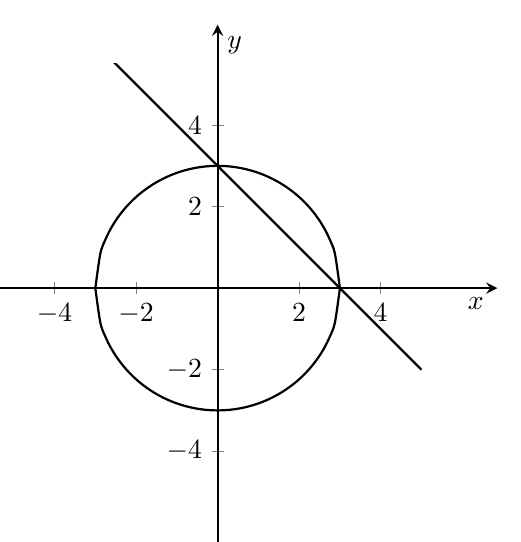
\begin{tikzpicture}
\begin{axis}[ 
xlabel=$x$,
ylabel=$y$,
axis x line=center, xlabel style={anchor=north west},
axis y line=center, ylabel style={anchor=south west},
xmin=-4.5,
xmax=5.9,
ymin=-5.5,
ymax=5.5,
axis line style={thick, shorten > = -0.5cm, shorten < = -0.5cm},
samples=50,
unit vector ratio*=1 1,
]

\addplot [domain=-3:3, thick, black, smooth]{sqrt(9-x^2)};
\addplot [domain=-3:3, thick, black, smooth]{-sqrt(9-x^2)};
\addplot [domain=-5:5, thick, black, smooth,]{3-x};

\end{axis};
\end{tikzpicture}}\\
    \subfloat[$C-(A \cup B) $]{\begin{tikzpicture}
\begin{axis}[ 
xlabel=$x$,
ylabel=$y$,
axis x line=center, xlabel style={anchor=north west},
axis y line=center, ylabel style={anchor=south west},
xmin=-4.5,
xmax=5.9,
ymin=-5.5,
ymax=5.5,
axis line style={thick, shorten > = -0.5cm, shorten < = -0.5cm},
samples=50,
unit vector ratio*=1 1,
]



\coordinate (A) at (axis cs:6,-3) {};
\coordinate (B) at (axis cs:-4,7) {};
\coordinate (C) at (axis cs:-4,9) {};
\coordinate (D) at (axis cs:6,9) {};
       \coordinate (At) at (axis cs:0,0) {};
\coordinate (Bt) at (axis cs:0,-6) {};
\coordinate (Ct) at (axis cs:9,-6) {};
\coordinate (Dt) at (axis cs:0,3) {};
\path[ pattern={Lines[
                  distance=2mm,
                  angle=45
                 ]},
        pattern color=gray!50](At)--(Bt)--(Ct)--(Dt);
\addplot [domain=-3:3, thick, black, smooth,fill=white]{sqrt(9-x^2)};
\addplot [domain=-3:3, thick, black, smooth,fill=white]{-sqrt(9-x^2)};
\addplot [domain=-5:5, thick, black, smooth]{3-x};
\draw [](axis cs:-4,0)--(axis cs:4,0);
\draw [](axis cs:0,4)--(axis cs:0,-4);
\end{axis};
\end{tikzpicture}}
    \subfloat[$(C-A)\cap (C-B)$]{\begin{tikzpicture}
\begin{axis}[ 
xlabel=$x$,
ylabel=$y$,
axis x line=center, xlabel style={anchor=north west},
axis y line=center, ylabel style={anchor=south west},
xmin=-4.5,
xmax=5.9,
ymin=-5.5,
ymax=5.5,
axis line style={thick, shorten > = -0.5cm, shorten < = -0.5cm},
samples=50,
unit vector ratio*=1 1,
]



\coordinate (A) at (axis cs:6,-3) {};
\coordinate (B) at (axis cs:-4,7) {};
\coordinate (C) at (axis cs:-4,9) {};
\coordinate (D) at (axis cs:6,9) {};
       \coordinate (At) at (axis cs:0,0) {};
\coordinate (Bt) at (axis cs:0,-6) {};
\coordinate (Ct) at (axis cs:9,-6) {};
\coordinate (Dt) at (axis cs:0,3) {};
\path[ pattern={Lines[
                  distance=2mm,
                  angle=45
                 ]},
        pattern color=gray!50](At)--(Bt)--(Ct)--(Dt);
\addplot [domain=-3:3, thick, black, smooth,fill=white]{sqrt(9-x^2)};
\addplot [domain=-3:3, thick, black, smooth,fill=white]{-sqrt(9-x^2)};
\addplot [domain=-5:5, thick, black, smooth]{3-x};
\draw [](axis cs:-4,0)--(axis cs:4,0);
\draw [](axis cs:0,4)--(axis cs:0,-4);


\end{axis};
\end{tikzpicture}}\\
    \subfloat[$\sim(\sim A)$]{\begin{tikzpicture}
\begin{axis}[ 
xlabel=$x$,
ylabel=$y$,
axis x line=center, xlabel style={anchor=north west},
axis y line=center, ylabel style={anchor=south west},
xmin=-4.5,
xmax=5.9,
ymin=-5.5,
ymax=5.5,
axis line style={thick, shorten > = -0.5cm, shorten < = -0.5cm},
samples=50,
unit vector ratio*=1 1,
]


\addplot [domain=-3:3, thick, black, smooth,pattern={Lines[
                  distance=2mm,
                  angle=-45
                 ]},
        pattern color=gray!50]{sqrt(9-x^2)};
\addplot [domain=-3:3, thick, black, smooth,pattern={Lines[
                  distance=2mm,
                  angle=-45
                 ]},
        pattern color=gray!50]{-sqrt(9-x^2)};
\end{axis}
\end{tikzpicture}}
%\caption{}
\label{fig:fig_p8b}
\end{figure}
$$\blacklozenge$$

\subsection{}
\begin{tcolorbox}
On the basis of the sketches made in the previous exeercise, formulate a proposition about relation that exist concerning complementation, union, and intersection. Try out your conjecture on other examples. In subsequent exercises you will be asked to try to prove such conjectures.
\end{tcolorbox}
\begin{align*}
\begin{array}{ll}
 1.4.2\, (a)\text{ and } (d) &A\cup(B\cup C)= (A\cup B)\cup C)\\
 1.4.2\, (b)\text{ and } (c)& A\cap(B\cup C)= (A\cap B)\cup (A\cap C)\\
 1.4.2(e)\,\text{ and }(f) &A\cup (B\cap C)= (A\cup B)\cap (A\cup C)\\
  1.5.1(a)\,\text{ and }(g) &\sim(A\cap B)=(\sim A)\cup(\sim B)\\
  1.5.1(h)&(\sim A)\cap A=\emptyset\\
  1.5.1(i)\,\text{ and }(j) &C-(A\cup B) = (C-A)\cap (C-B)\\
    1.5.1(k)&\sim (\sim A)=A\\
\end{array}
\end{align*}
$$\blacklozenge$$
\newpage

 \section{Set identities and other set relations}
\subsection{}
\begin{tcolorbox}
Prove that if $A\subset B$, then:
\begin{align*}
\begin{array}{ll}
(a)&A\cap C \subset B \cap C\\
(b)& \sim B \subset \, \sim A\\
(c) &A \cap B = A\\
(d) &A \cup C \subset B\cup C\\
\end{array}
\end{align*}
\end{tcolorbox}
\textbf{a)}$\quad A\cap C \subset B \cap C $\\\\
Given is $x\in B$ if $x \in A$. Suppose $x \in A\cap C$, then $x \in A$ (given) and $x \in C$ but $x \in B$ (given) and as $x \in C$ follows that $x \in B\cap C$. And we conclude that $A\cap C \subset B\cap C$. \\\\
$$\lozenge$$
\textbf{b)}$\quad \sim B \subset \, \sim A$\\\\
Given is $x\in B$ if $x \in A$. If $x\not\in B$ then $x\in \, \sim B$. As $A\subset B$, $x$ will not be in $A$ but $x\in \sim A$. So $x\in \, \sim B \Rightarrow \quad x\in \, \sim A$ and thus $\sim B \subset \, \sim A$. \\\\
$$\lozenge$$

\textbf{c)}$\quad A \cap B = A$\\\\
Given is $x\in B$ if $x \in A$. Suppose $x \in A\cap B$, then $x \in A$ and thus $A\cap B \subset A$. Suppose $x \in A$, then $x \in B$ as $A\subset B$ and thus $x\in A\cap B$ from which we conclude $A \subset A\cap B$.
$$\lozenge$$
\textbf{d)}$\quad A \cup C \subset B\cup C$\\\\
Given is $x\in B$ if $x \in A$. Suppose $x \in A\cup C$, then $x \in A$ or $x\in C$. But $x\in B$ (given), so $x\in B$ or $x\in C$ and thus $x\in B\cup C$, from which we conclude $A\cup C \subset B\cup C$.
$$\blacklozenge$$
\newpage
\subsection{}
\begin{tcolorbox}
Verify that each of the following is an an identity:
\begin{align*}
\begin{array}{ll}
(a)&A\cup \emptyset = A\\
(b)& A\cap \emptyset = \emptyset\\
(c) &A \cap A = A\\
(d) &A \cup A =A\\
(e)&(A\cup B)\cup C= A\cup(B\cup C) \\
(f)& (A\cap B)\cap C= A\cap(B\cap C)\\
(g) &A\cup (B\cap C)= (A\cup B)\cap (A\cup C)\\
(h) &X-(A\cup B) = (X-A)\cap (X-B)\\
(i)&A\, \cap \, \sim A = \emptyset\\
(j)& A\, \cup \, \sim A = U\\
\end{array}
\end{align*}
\end{tcolorbox}
\textbf{a)}$\quad A\cup \emptyset = A $\\\\
This is a consequence of remark 3.3 page 7: the empty set $\emptyset$ is a subset of every set. So, $\emptyset\subset A$ giving the asked identity. \\\\
$$\lozenge$$
\textbf{b)}$\quad A\cap \emptyset = \emptyset$\\\\
If $x\in A\cap \emptyset$ then $x\in \, A$ and $x$ must also be in $\emptyset$ which is impossible by definition. So there is no element $x \in \emptyset$ which can satisfy $x\in A\cap \emptyset$ giving the proposed identity. \\\\
$$\lozenge$$
\textbf{c)}$\quad A \cap A =A$\\\\
 Suppose $x \in A\cap A$, then $x \in A$ and $x\in A$ and thus $x\in A$, giving  $ A \cap A \subset A$. Suppose $x \in A$, then obviously  $x \in A$ and $x \in A$, giving $A\subset A\cap A$. Hence $A \cap A =A$
$$\lozenge$$
\textbf{d)}$\quad A \cup A =A$\\\\
Suppose $x \in A\cup A$, then $x \in A$ or $x\in A$ and thus $x\in A$, giving  $ A \cup A \subset A$. Suppose $x \in A$, then obviously  $x \in A$ or $x \in A$, giving $A\subset A\cup A$. Hence $A \cup A =A$
$$\lozenge$$
\textbf{e)}$\quad (A\cup B)\cup C= A\cup(B\cup C) $\\\\
 Suppose $x \in (A\cup B)\cup C$, then $x \in (A\cup B)$ or $x\in C$ and thus $x\in A$ or $x\in B$ or $x\in C$. So  $x\in B$ or  $x\in C$  can be written as $x\in (B\cup C)$. So $x\in A$ or $x\in (B\cup C)$, giving $(A\cup B)\cup C\subset A\cup(B\cup C)$. The same reasoning yields for $x\in A\cup(B\cup C)$ giving the identity.
$$\lozenge$$
\textbf{f)}$\quad (A\cap B)\cap C= A\cap(B\cap C)$\\\\
 Suppose $x \in (A\cap B)\cap C$, then $x \in (A\cup B)$ and $x\in C$ and thus $x\in A$ and $x\in B$ and $x\in C$. So  $x\in B$ and  $x\in C$  can be written as $x\in (B\cap C)$. So $x\in A$ and $x\in (B\cup C)$, giving $(A\cap B)\cap C\subset A\cap(B\cap C)$. The same reasoning yields for $x\in A\cap(B\cap C)$ giving the identity.
$$\lozenge$$
\textbf{g)}$\quad A\cup (B\cap C)= (A\cup B)\cap (A\cup C)$\\\\
 Suppose $x \in A\cup (B\cap C)$, then $x \in A$ or $x\in (B\cap C)$.  Take the case $x\in A$, then  $x\in A\cup B$ and  $x\in A\cup C$ which implies $x\in (A\cup B)\cap (A\cup C)$, giving $A\cup (B\cap C)\subset (A\cup B)\cap (A\cup C)$. The other case:  if $x\in B\cap C$ then $x\in B$ and $x\in C$. So, $x \in A\cup B$ and $x\in A\cup C$ giving also $A\cup (B\cap C)\subset (A\cup B)\cap (A\cup C)$.\\
 On the other hand,  be $x \in (A\cup B)\cap (A\cup C)$ then $x \in (A\cup B)$  and $x \in (A\cup C)$. Let's first take the case $x\in A$ then obviously $x\in A\cup (B\cap C)$ even if $x\not\in  B\cap C$. Alternatively, be $x\not \in A$ then we must have $x \in B$ and $x\in C$ which implies $x\in B\cap C$, giving again $x\in A\cup (B\cap C)$.
$$\lozenge$$
\textbf{h)}$\quad X-(A\cup B) = (X-A)\cap (X-B)$\\\\
 Suppose $x\in X-(A\cup B)$, then $x \not\in A$ and $x \not\in B$ which implies $x \in X-A$ and $x \in X-B$ and thus $x \in X-A\cap X-B$ giving $X-(A\cup B) \subset (X-A)\cap (X-B)$.\\
 The other way around. Suppose $x\in(X-A)\cap (X-B)$. Then $x\in(X-A)$ and $x\in(X-B)$ which implies  $x\not \in A$ and $x\not \in B$ giving $x\not \in A \cup B$ which in turn implies $x\in X-(A\cup B)$ giving $(X-A)\cap (X-B)\subset  X-(A\cup B)$.\\Conclusion: $ X-(A\cup B) = (X-A)\cap (X-B)$
$$\lozenge$$
\textbf{i)}$\quad A\, \cap \, \sim A = \emptyset$\\\\
 Suppose $x\in A\, \cap \, \sim A$, then $x \in A$ and $x \not\in A$ which is a contradiction, so the only element which is always an element of any set is the empty set, so $ A\, \cap \, \sim A \subset \emptyset$. Suppose on the contrary that $x\in\emptyset$. This implies that $x$ correspond to the empty set and as the empty set is an element of any set, we have  $\emptyset \subset A\, \cap \, \sim A  $
$$\lozenge$$
\textbf{j)}$\quad A\, \cup \, \sim A = U$\\\\
 Suppose $x\in A\, \cup \, \sim A$, then $x \in A$ or $x \not\in A$. So, in any case $x\in U$ and thus $A\, \cup \, \sim A \subset U$.\\
 On the opposite way  suppose that $x\in U$. Then obviously $x\in A$ or $x\in \sim A$ and thus $U\subset A\, \cup \, \sim A$.
$$\blacklozenge$$
